\documentclass{report}

%PACKAGES
\usepackage{hyperref}
\usepackage[usenames,dvipsnames]{color}
\usepackage{graphicx}
\usepackage{amsmath}
\usepackage{tabularx}
\usepackage{enumerate}
%USEFULL COMMAND
\newcommand\myworries[1]{\begin{center}\textcolor{red}{#1}\end{center}}
\title{EPFL semester project\\Extraction of Protein Concentration from Scientific Literature}
\author{Phil\'emon Favrod\\\\Supervisors: Jean-C\'edric Chappelier, Renaud Richardet}

\begin{document}
	\maketitle
	\tableofcontents
	\chapter{Introduction}
	

		\section{Motivation}
		\label{sec:motivations}
		A usual start for a paper in the field of Information Extraction (IE)
		is the assessment of the increasing difficulty to access data hidden, 
		for instance, in texts or, more generally, in unstructured form. The
		growth of scientific publication is exponential. For instance,
		the world-known biomedical citation database, Pubmed, contains over 		
		20-millions (2010) citations while it contained less than 8-millions
		citations in the mid-eighties\footnote{\url{http://database.oxfordjournals.org/content/2011/baq036.full}}. 
		That is, looking for very specific data is a problem that can only
		become harder. For instance, the use of automated techniques such as the ones
		coming from the natural language processing (NLP) are needed to
		keep the access time to specific data realistic. The Blue Brain 
		project\footnote{\url{http://bluebrain.epfl.ch}} (BBP)
		where simulation of biological models requires a lot of very precise
		data is not a departure from that norm. In the latter context, the
		researchers' need to access information concerning protein 
		concentration at different scale in the brain is the main motivation of this
		project. In the point of view of the Computer scientist, as described later, it
		is also a trial to extract very specific pieces of data using simple extraction
		model. Therefore, the results of this approach is valuable for future research
		in that field even though its very specialized character limits the significance
		of generalizing to other fields.
		
		
		\section{Project description}
		\label{sec:project_desc}
		The project falls within the line of successive works in natural language processing
		at the Blue Brain project. For two years, IE tools have been developed for different 
		purposes, mainly to achieve named entity recognition (NER) for neuroscience extending the Apache 
		UIMA framework\footnote{\url{http://uima.apache.org}} and giving birth to the Bluima 
		toolkit. Henceforth, using these
		tools to perform Relation Extraction (RE) and construct accessible databases for 
		researchers is the ultimate purpose in which this project take place. 
		Taking advantage of building upon this past work, this semester work focuses on building an analysis chain
		to put in relation mentions of proteins, concentrations and their local context such
		as brain regions, cell types or subcells. In more practical terms, this project is about
		building a ready-to-use UIMA analysis chain to extract triplets containing a protein
		mention, its associated concentration and the biological location of those two. In the next
		chapters, the term ``triplet'' will be used to refer to this kind of piece of data.
		
		\paragraph{}In order to more precisely describe the problem, we will
		consider an example. Consider the following sentence [PMID: 15659591]:
		
		\begin{quotation}
		Using this calibration procedure, we find that mature granule cells (doublecortin-) contain approximately 40 $\mu$M, and newborn granule cells (doublecortin+) contain 0-20 $\mu$M calbindin-D28k. 
		\end{quotation}
		
		The latter describes a strong relation in the sense that it establishes 
		how concentrated are ``calbindin-D28k'' proteins in ``granule cells''.
		Nevertheless, this relation is mentionned in an unstructured form. This
		information would be more accessible if it was in a more structured 	
		format such as:
		\begin{center}
			\begin{tabular}{|l|l|l|}
				\hline
				\textbf{Protein} & \textbf{Concentration} & \textbf{Location}\\
				\hline
				calbindin-D28k & 40 $\mu$M & mature granule cells (doublecortin-)\\
				\hline
				calbindin-D28k & 0-20 $\mu$M & newborn granule cells (doublecortin+)\\
				\hline
			\end{tabular} 
		\end{center}
		This transformation (from unstructured form to structured form) of such 
		a relation is the main goal of this project. We will refer to this kind
		of transformation by calling it an extraction, as it is usually done in 
		IE. The columns (protein, concentration and location) of the table are 
		the named entities taking part in the
		relation. The above type of relation, 
		describing how concentrated a protein is in a brain location, will be
		referred to as the targeted relation to distinguish it from
		other kind of relations that will appear in our 
		results and because it is what the researchers are mainly looking for.  
		
		\paragraph{}Chapter \ref{chap:overall_model} will focus on the methodological aspect
		of this project by describing how the tool aiming to perform the above 
		transformation was developed and how it works. Then, the results of
		large-scale extractions are analyzed in chapter \ref{chap:results}.
		Finally, a conclusion can be found in chapter \ref{chap:conclusion}.
	            
                \chapter{The process: building the UIMA chain}
                \label{chap:overall_model}
                
                This chapter intends to explain the design decisions which leads to the final
				tool developed during this project. First, a little digression
				is made in order to describe the main challenge(s) we had to face.
				Then, the method used to extract the text from PDF documents is
				explained. Finally, the entire UIMA analysis chain will be 
				described component by component. 
				
				\section{Facing the absence of any annotated corpus}
		The greatest obstacle this project has to overcome from the start
		is the absence of a reference gold standard, i.e. the absence of
		an already-annotated corpus. Annotated corpora for biomedical entity exist and some key components this project is
		built upon are themselves built on machine learning
		model and trained on such corpora (see sections \ref{sec:preprocessing}, 
		\ref{sec:annot_prot} or \ref{sec:locations}). However, it appears that no annotated corpus includes
		information regarding the targeted relation (see section \ref{sec:project_desc}). 
		Furthermore, no annotated corpus seems to
		exist even for the sub-relation between a protein mention and a concentration mention. 
		The work of annotating such entities in a corpus is outside the field of NLP and Computer
		science; it implies the involvement of individual(s) specialized in the field in question ---
		(neuro)biologists in the present case. Due to the lack of annotated data, 
		supervised machine learning cannot be considered as a design option. That is, the relation extraction processes designed along this project could only be 
		rule-based heuristics or unsupervised methods. 
		
		\paragraph{}Note that the absence of any such corpus also significantly
		affects the evaluation method. That is, even if we tried to be
                the more quantitative we could in our decision path, some decision had to be taken only on a totally
                qualitative basis. Another problem the lack of corpus induces in evaluation is the absence of
                idea concerning the recall of our heuristics since the denominator of the recall formula remains
                unknown. Therefore, the chosen approach in this project was to incrementally improve the precision
                of our tools while qualitatively judging whether the decision taken were too specific or not.
				
				
				
					
				\section{Extracting the full text from PDF}
				Some considerations must be taken into account regarding the 
				corpora that can be used and how they can. The NLP tasks 
				conducted in the BBP are currently performed on either
				the abstracts of scientific publications or on the full-text PDFs 
				of the scientific publications\footnote{More
				precisely, the abstracts and PDFs from PubMed. See \url{http://www.ncbi.nlm.nih.gov/pubmed}.}. Preliminary
				analysis of abstracts quickly leads to the conclusion that a data 
				as specific as the concentration of proteins hardly
				appears in abstracts. We therefore choose to run our tool on the
				full-text PDFs. Thus, ``PDF reader''
				converting PDFs to raw text are used in this project. For that matter, we used the toolkit developed during
				another semester project \cite{rollier} which is a version of PDFTextStream\footnote{See \url{http://snowtide.com/}} specialized in the extraction of scientific content.	
				
				
				
				\section{A quick overview of the analysis chain}
				
				Before describing each component of the UIMA chain, we will just 
				look at the big picture of the chain shown in figure \ref{fig:global_pipeline}. As one could expect, the design of our chain follows 
				the usual pattern used in relation extraction:
				
				\begin{itemize}
					\item	the text is preprocessed simplifying it enough to make it suitable for the
							rest of the chain; this includes tokenization, POS tagging, lemmatization
							and chunking;
					\item	the NERs are applied to annotate the underlying instance of the relation
							in question (here: protein, concentration and a brain location);
					\item	the relation extraction algorithm is applied to those named entities;
					\item	finally, some filtering is applied to clean up the results.
				\end{itemize}
                
                \begin{figure}[h]
					\centering
					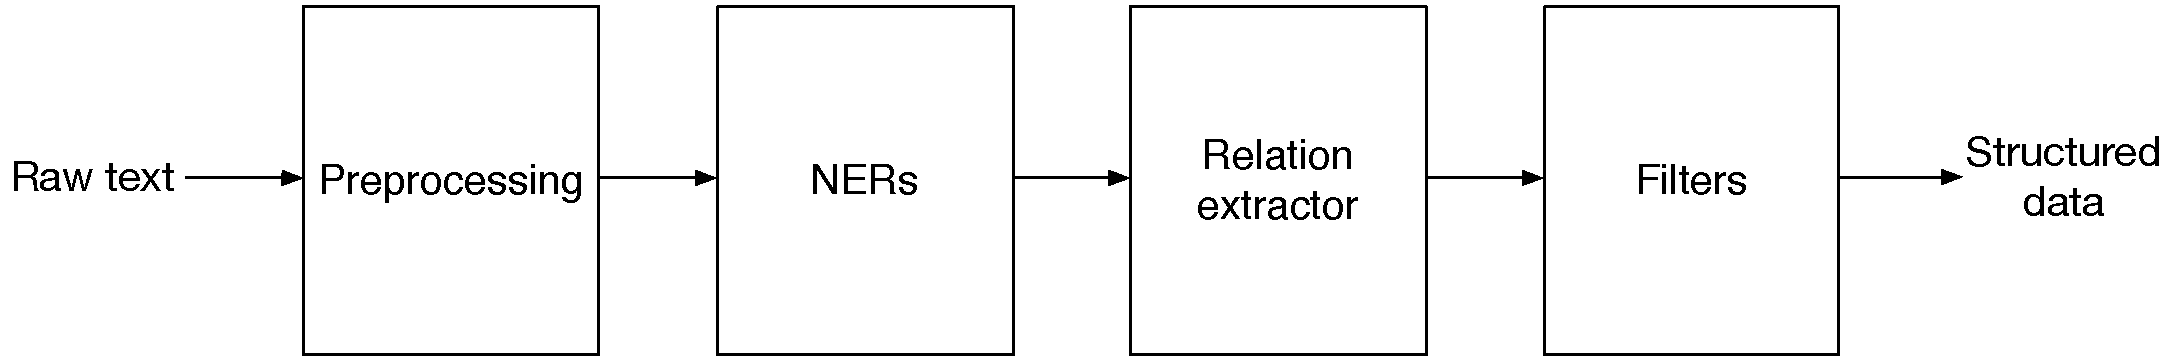
\includegraphics[width=\textwidth]{fig/global_pipeline.pdf}
					\caption{The big picture of the processing chain}
					\label{fig:global_pipeline}
                \end{figure}
                
                \section{Preprocessing}
                \label{sec:preprocessing}
                The first stage of the UIMA chain is to treat the text such
                that it can be used by usual NLP tools (see Figure \ref{fig:preprocessing}). First, the text is
                sliced into sentences
                and words are tokenized. Then, each token is assigned its corresponding part-
                of-speech. Then, the sentences are syntactically chunked. All these tasks are
                achieved using the JulieLab NLP tool suite\footnote{\url{http://www.julielab.de/}} which consists
                of UIMA wrappers for the Apache OpenNLP library\footnote{\url{http://opennlp.apache.org/}}. 
                Finally, the token are lemmatized using BioLemmatizer \cite{biolemmatizer}.

                \begin{figure}[h]
                  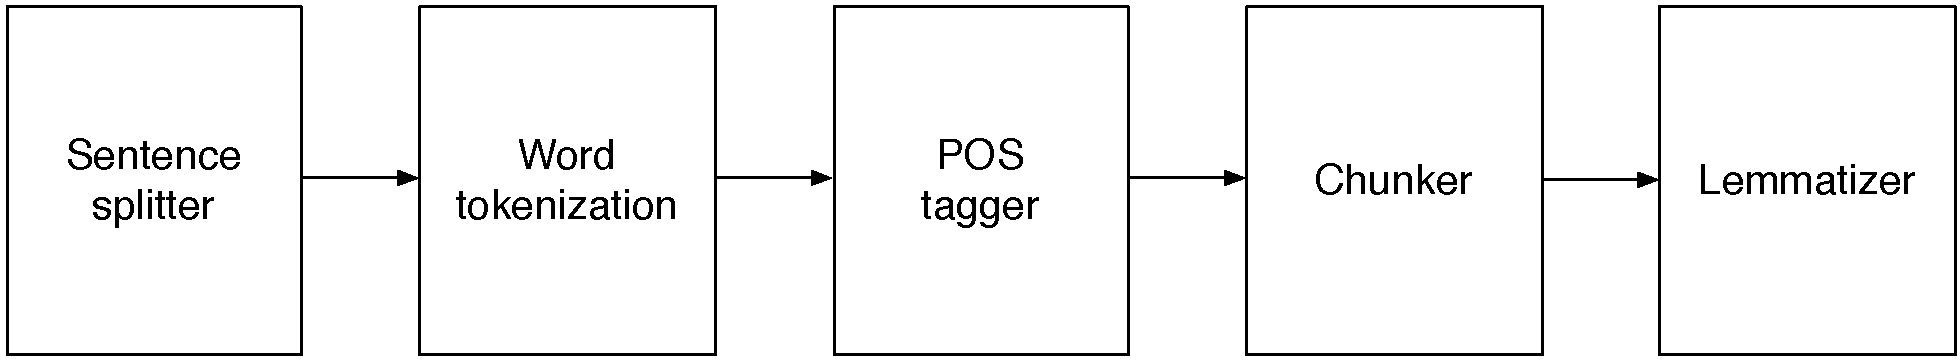
\includegraphics[width=\textwidth]{fig/preprocess_diagram.pdf}
                  \caption{The different components of the preprocessing pipeline.}
                  \label{fig:preprocessing}
                \end{figure}

                For example, given the sentence ``The man walked in the night.'', it is first recognized as
                a sentence by the JulieLab-OpenNLP Sentence Splitter. Then, its words are tokenized
                using again a JulieLab-OpenNLP tool. In our example, the sentence is simplified as 
                a sequence of tokens as follows:
                
                \begin{center}
					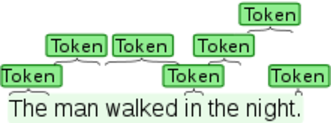
\includegraphics[width=.45\textwidth]{fig/brat_tokenizer_output.pdf}
				\end{center}
				Then, each token is assigned its presumed grammatical role in the sentence (a
				part-of-speech tag) by the JulieLab-OpenNLP POS Tagger. For instance,
				
				\begin{center}
					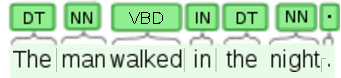
\includegraphics[width=.45\textwidth]{fig/brat_pos_tagger_output.pdf}
				\end{center} where \texttt{DT} stands for determinant, \texttt{NN} for a singular noun,
				\texttt{VBD} for a verb (past tense) and \texttt{IN} for a preposition. Then, this POS tags
				are grouped into grammatical chunks: 
				
				\begin{center}
					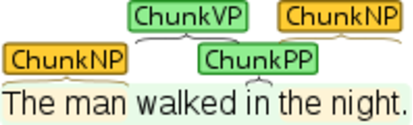
\includegraphics[width=.45\textwidth]{fig/brat_chunker_output.pdf}
				\end{center}
				Finally, the BioLemmatizer \cite{biolemmatizer} sets the lemmas of the token's instances. In the above example, it has the only effect to assign the lemma
				``walk'' to the token ``walked'', the lemma of the other tokens
				being themselves.
				
				\section{The Named Entity Recognizers}
				The second stage of the UIMA pipeline consists in detecting the occurrence
				of the named entities which matter in the context of the project. Since the
				approach is very different depending on the named entity in question, each
				subsection below describes the model used to annotate a particular named entity.
				
				\subsection{Annotating the Concentrations}
				\begin{figure}[h!]
					\centering
					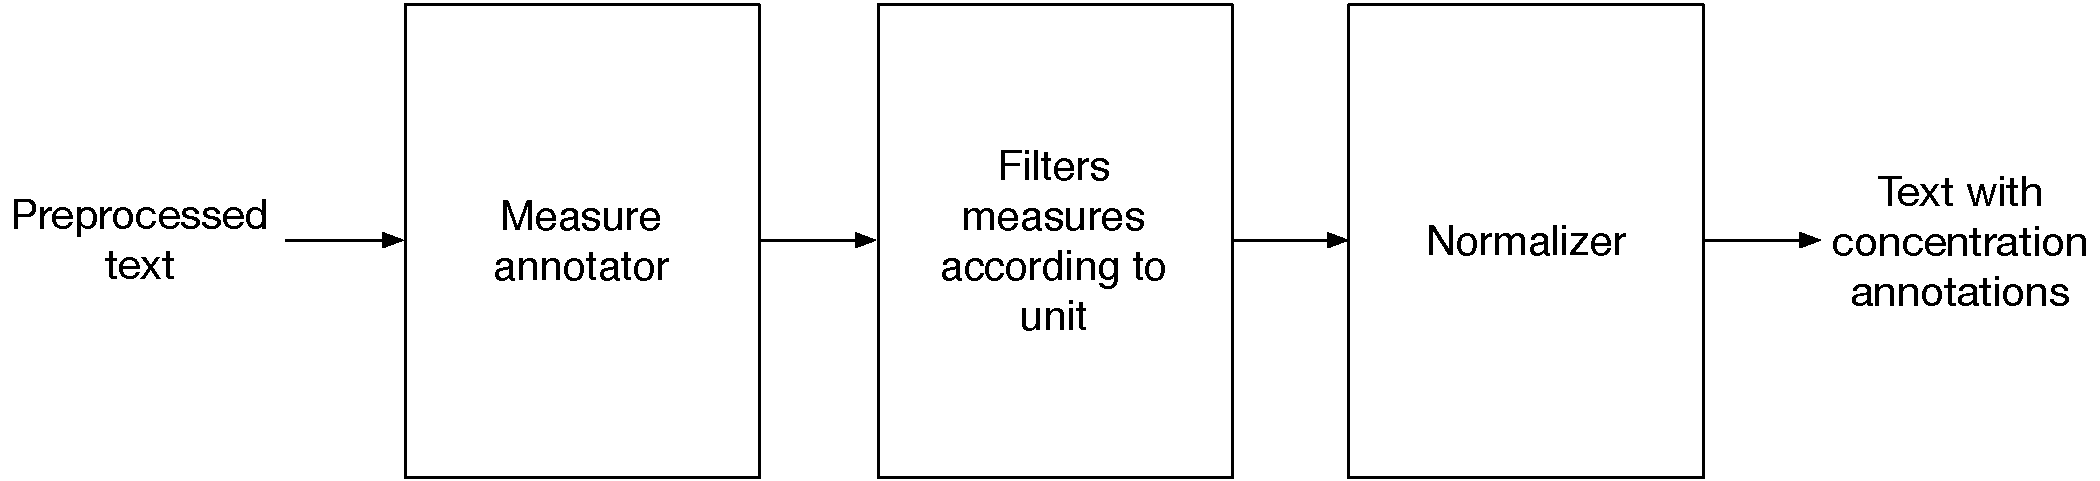
\includegraphics[width=\textwidth]{fig/concentration_pipeline.pdf}
					\caption{The overall pipeline for annotating concentrations}
					\label{fig:concentration_pipeline}
				\end{figure}
				
				Concentrations constitutes obviously a class of named entity of great interest in this project. 
				Such a class is a subset of a larger class, 
				the measures for which the Bluima toolkit \cite{bluima} provides a
                regexp-based annotator developed during another semester project 
                \cite{portmann} at the BBP to detect the mentions of any
                kind of measurements. It extracts the measures as a pair whose 
                first element is the value and the second one is the unit. For 
                instance, ``1 $\mu$g/ml'' is extracted as $\{$1, ``$\mu$g/ml''$\}$. 
                
                The concentration NER is built upon this tools  by filtering 
                out the measures which have no unit or a unit which does not 
                correspond to a concentration measurement. The unit in question
                includes measures of molarity, ratios between a measure of weight 
                and a measure of volume and other specific concentration units.
				
				\subsection{Normalizing the Concentrations}
				\paragraph{}The first results reveals the need to normalize the
				unit of concentration. Otherwise, for instance, ``0.005 mg/mL insulin'' 
				would be considered a different concentration of insulin than 
				``5 mg/L insulin'' while, physically speaking,
				$$0.005 [\textup{mg/mL}] = 5 [\textup{mg/L}].$$
				To explain such a need, note that, the model of relation extraction being 
				based on co-occurrences, the frequency of a co-occurrence is a 
				valuable information but, since measures of concentration 
				are not necessarily normalized in the text, some concentrations 
				may be considered as different while they are the same. To solve
				that matter, we consider three classes of concentrations units, 
				namely
                
                \begin{enumerate}[1.]
					\item the units expressed in terms of molarity (molar, mol/m3 , etc.),
					\item the units expressed as a ration of a weight and a volume (like mg/ml, kg/l, etc.) and
					\item the other specialized units (like ppm, ppb, etc.)
				\end{enumerate}
								
				After having characterized as concentration each measure whose 
				unit is a member of one of those classes. The ones that can be 
				normalized, namely classes 1 and 2, are normalized using a
				regexp-based algorithm. Every units in the first category can be 
				converted to a similar unit. The
				most logical choice is the standard unit used among researchers, 
				namely molar\footnote{i.e. mol/L, sometimes abbreviated by M. See
				\url{http://en.wikipedia.org/wiki/Molar_concentration} for more
				details.}. Note that the second class of units cannot be 
				converted into the first one without any knowledge of the context,
				since it requires the knowledge of the molar mass to perform such 
				a conversion\footnote{It is outside the scope of this project, 
				but this is not an unrealistic goal given an appropriate database
				to look up the molar masses.}.
				However, such a class of unit can be normalized inside itself. 	
				Therefore, kg/m$^3$ was chosen as targeted unit when normalizing the second 
				class of units.
				
				\paragraph{}The normalization is performed using a regex-based 
				approach. First, each SI prefix (such as d-, nano- or $\mu$-) is
				mapped to the power of 10 it corresponds to so that we can get
				standardized unit. For instance, the value of concentration whose unit 
				are prefixed by $\mu$- are multiplied by $10^{6}$. 
				Then, for the second class, we convert volume units (i.e. their 
				denominator). In spite of its simplicity,
				this approach seems to result in good qualitative results. 
				Table \ref{tab:concentration} 
				shows some examples of unit transformation performed by the 
				normalizer.
				
				\begin{table}[h!]
					\centering
					\begin{tabular}{|l|l|}
						\hline
						\textbf{Before normalization} & \textbf{After normalization}\\
						\hline
						10 nM & 10$^{-8}$ molar\\
						10 mM & 0.00001 molar\\
						163 g/m$^3$ & 0.163 kg/m$^3$\\
						245.6 ng/ml & 0.0002456 kg/m$^3$\\
						\hline
					\end{tabular}
					\caption{Examples of unit normalization for concentrations}
					\label{tab:concentration}
				\end{table}
                
                \section{Annotating the Proteins}
                \label{sec:annot_prot}
                
                Another significant existing work this project need and is built 
                upon is a protein NER. This section describes how we selected it
                among the two protein NERs provided by the Bluima toolkit \cite{bluima} and how we adapted it to our needs.
                
                \subsection{BANNER}
                We first considered BANNER \cite{banner}, a protein NER that has
                been adapted for UIMA. It is based on a machine learning model 
                (Conditional Random Field).
                        \subsubsection{BANNER tokenization weakness} 
                        First experimental results suggest that BANNER is likely to mistokenize
                        protein mentions in presence of measure mentions. To illustrate the problem, consider the
                        following sentence [PMID: 19535906]:
                        
                        \begin{quote}
                        Cells were lysed in a buffer containing 50 mM Tris at pH 7.5, 1\%~Triton X-100, 150 mM NaCl, 
                        5 mM EDTA, 1 mg/ml pepstatin A, 1~$\mu$g/ml leupeptin, 2 $\mu$g/ml aprotinin, 1 mM PMSF, 
                        0.1 mg/ml benz- 21. amidine and 8 g/ml each of calpain I and calpain II. 
                        \end{quote}

                        The result of BANNER annotation is:
			
                        \begin{quote}
                        [...], 1 mg/ml $\underbrace{\text{pepstatin A, 1 }\mu\text{g}}_{\text{PROTEIN}}$/$\underbrace{\text{ml leupeptin}}_{\text{PROTEIN}}$, 2 $\mu$g/ml aprotinin, 1~mM PMSF, [...]
                        \end{quote}

                        As one can see, the bounds of the annotations returned by BANNER exceeds the protein mentions. 
                        In other words, such annotations cover
                        some part of the surrounding measures in the text. Note that some other protein mention such as ``aprotinin'' are not detected by
                        BANNER. 
					\subsection{Benchmark of BANNER against Gimli}
					
                    \begin{figure}[h]
						\centering
						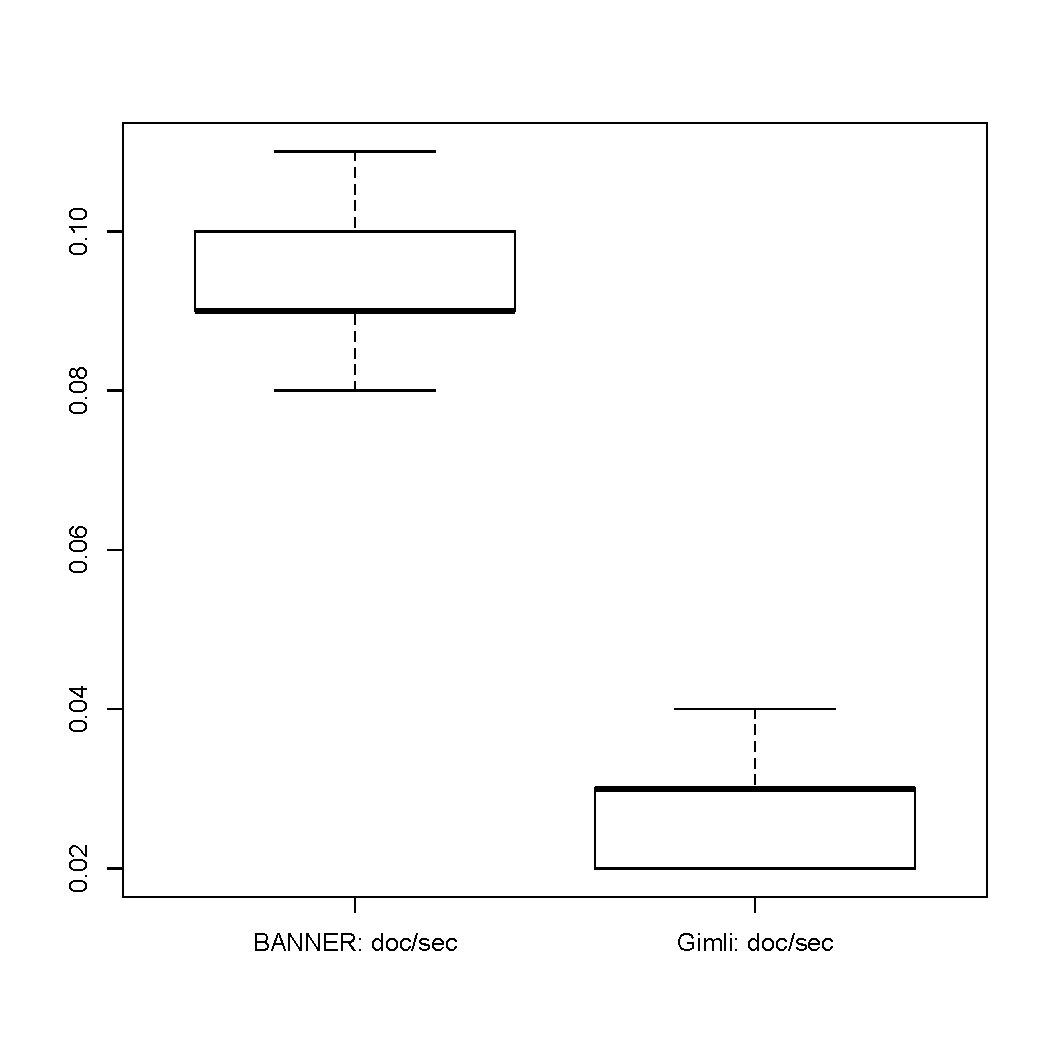
\includegraphics[width=\textwidth]{fig/banner_gimli_bm_docs.pdf}
						\caption{Comparative boxplot of speed performance between Banner and Gimli}
						\label{fig:doc_per_sec}
					\end{figure}
					
                                        
                    The above-mentioned problem in BANNER leads us to study one 
                    of its competitor, Gimli \cite{gimli}, another machine-learning-based NER for the recognition of protein mentions.
                    The quality of its
					output appeared qualitatively better than the one of BANNER; 
					since no similar tokenization problem were 
					found. However, it runs
					remarkably slowly compared to BANNER and it is only partially 
					integrated with UIMA. A major argument in favor of Gimli
					was that its ability to do syntactical parsing, 
					which could have been reused later. However, because of its
					incomplete UIMA integration, these data could not be trivially accessed and reused. 
					Moreover, the incomplete integration of Gimli into UIMA seems buggy: it enters a dead lock
					after annotating about ten PDFs.
					
					The boxplots
					on figure \ref{fig:doc_per_sec} compare BANNER and Gimli 
					performances in terms of the number of documents processed by 
					second. This data have been collected by profiling both 
					annotators while they were 
					analyzing PDFs articles. As one can see, according to this 
					dataset, BANNER ($M = 0.094$ doc/s) is on average 
					about three times quicker than Gimli ($M=0.027$ doc/s). That 
					is, BANNER analyzes about 338 documents
					in one hour on average while Gimli analyzes only about 97 of 
					them. Considering the decrease in the runtime involved by the use of  Gimli 
					while running on a huge number of documents and the
					time spent to debug and to fully integrate it to UIMA leads us
					to keep BANNER as protein NER and to improve its results.
					
					
					
					
					\subsection{BannerM}
					\label{sec:bannerM}
                    To overcome the problem of tokenization of protein mentions
                    with BANNER, a wrapper was developed so that
                    BANNER is fed with a cleaned input. That is, all 
                    measurement mentions detected in the text are removed\footnote{More precisely, they are replaced by spaces.} 
                    before BANNER analyzes the text. 
                    This tool will be referred to as BannerM where the ``M'' stands for ``modified''.
                                        
                    \paragraph{}The surprising fact is that, once the measurements filtered out of the input, BANNER seems to recognize
                    more protein. For instance, in the sentence mentionned above, the ``aproptinin'' mention is recognized
                    as one. This is also reflected on larger datasets: 
                    when run on 238 PDFs, BannerM found 22613
                    distinct protein mentions while BANNER found only 22090. 
                    Moreover, they both recognize 19380
                                        distinct common entities, but, for 18599 of them, BannerM found more occurrences. Finally, considering the tail
                                        of the distribution of the length of the protein mentions, BannerM appears to have a closer distribution to the
                                        one of GENIA \cite{genia}, a reference protein-annotated corpus, (see section \ref{sec:genia} for more information about GENIA) than BANNER which still have a lot of very long protein mentions as one can see on
                                        figure \ref{fig:bannerVSbannerM}.

                                        \begin{figure}[h!]
                                          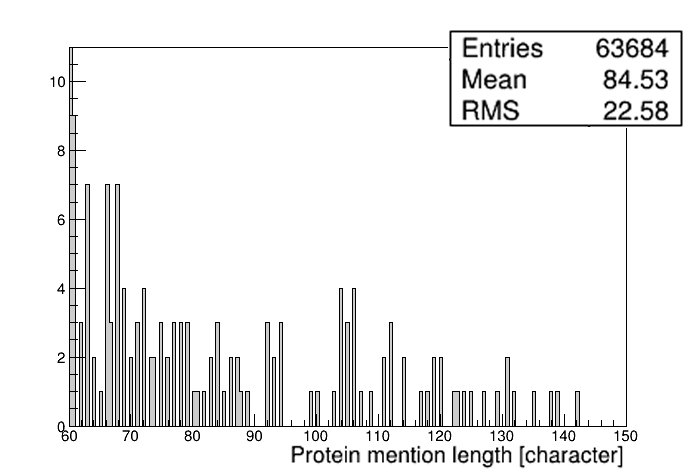
\includegraphics[width=.5\textwidth]{fig/banner_prot_length.png}
                                          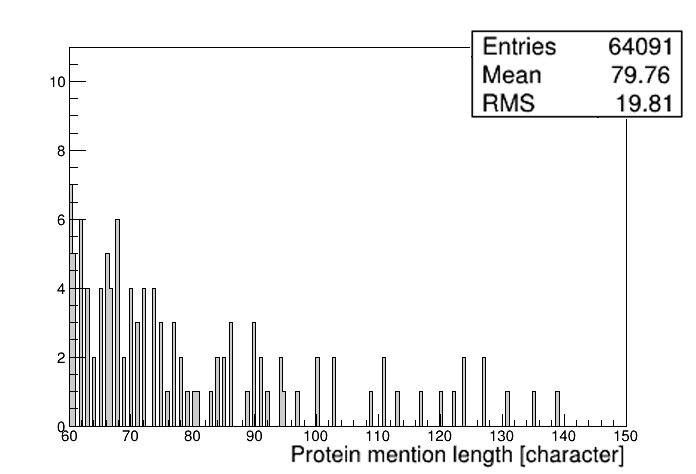
\includegraphics[width=.5\textwidth]{fig/bannerM_prot_length.png}
                                          \caption{Histograms of the distribution of length of protein mentions extracted by BANNER (top) 
                                            and BannerM(botom)}
                                          \label{fig:bannerVSbannerM}
                                        \end{figure}
                                        %%%%%%%%%%%%%%%%%%%%%%%%%%%%%%%%%
                
                \paragraph{}Using BannerM justifies the position of the protein NER 
                in the pipeline --- after the measurement and concentration 
                annotator. Therefore, it gets already annotated text with 
                mentions of measurements. Thus, BannerM
                can easily remove them before passing the text to the wrapped 
                original BANNER \cite{banner} version.       
                
               
                \subsection{Filtering on the length of Proteins}
                \label{sec:genia}
                The first results of protein annotations has shown that when 
                the sentence is not an English
                sentence --- this appends when the extraction of the full-text is 
                not valid --- machine-learning-based annotators,
                especially BANNER, becomes unpredictable. A qualitative analysis 
                leads to the fact that proteins with the longest
                length tends to be false positives. To find an upper bound for 
                protein name length, the already-annotated 
                mentions of proteins have been extracted from the GENIA 
                corpus~\cite{genia}. An histogram summarizing protein name length 
                can be found on figure \ref{fig:hist_genia}.  As the histogram 
                tail shows, the most 
                long protein mention found in the GENIA corpus has a length of 118 characters. The dataset being large enough to make decision
                using it, we set our cutoff point a bit higher to allow some
                variation, i.e. 150 characters. In other words, 
                BannerM implements a feature to filter out proteins estimated
                mentions whose length are greater than 150 characters.
                                               
                  \begin{figure}
                    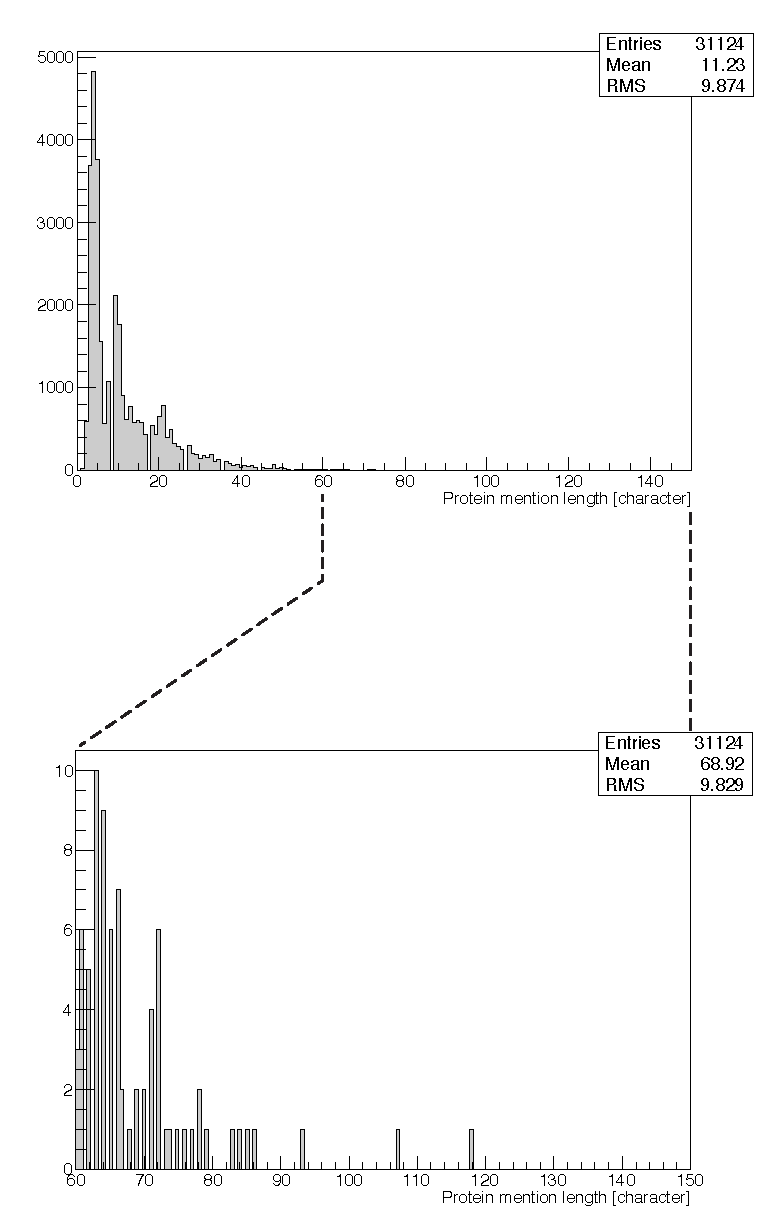
\includegraphics[width=0.9\textwidth]{fig/genia_dist.pdf}
                    \caption{Histograms summarizing the length of protein found in the GENIA corpus. 
                    Top: overall distribution of the length of protein mentions in the GENIA coups. 
                    Bottom: the tail of that distribution.}
                    \label{fig:hist_genia}
                \end{figure}
                         
                \section{Annotating the Brain Regions, Cell types and Subcells}
                \label{sec:locations}
                The annotator developed to detect the brain regions is a machine-learning-based
                annotator (CRF) \cite{br}. It is now a component of the Bluima analysis tools \cite{bluima}. It
                has been retrained for the purpose of this project. The
                annotators and subcells and cell types are list-based annotators 
                and, thus, should
                produce more primitive results. That is, a big part of the project focused on
                the triplets~$\{\text{protein, concentration, brain region}\}.$
                
                However, one should also consider cell types and subcells given
                the high level of precision induced by protein concentration. 
                The concentration of a protein makes more sense in the context of 
                a subcell or a cell type than in the context of a brain region. 
                The lack of targeted relations found in the extraction of the 
                latter form suggests that this intuition is correct.
                
		\section{The Relation Extraction Stage}
		\begin{figure}[hb]
		    \centering
		    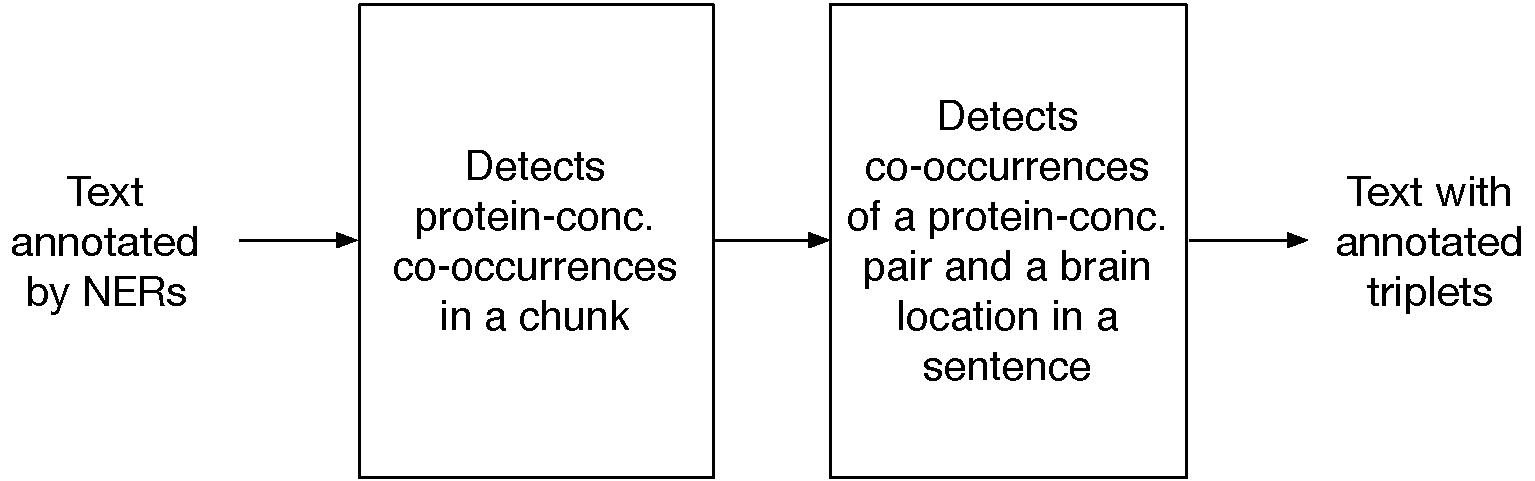
\includegraphics[width=0.8\textwidth]{fig/RE_diagram.pdf}
		    \caption{The overall model for relation extraction}
		    \label{fig:RE_model}
		\end{figure}
		Given the absence of any reference annotated corpora, the time 
		constraints and the lack of biomedical experience to annotate a corpus 
		ourselves, the approach used to extract relations is quite simple and 
		based on a co-occurrence model. Two named entities 
		co-occurrs in a given enclosing scope (e.g. sentence) if there is at 
		least one occurrence of the considered scope 
		in the text containing occurrences of both named entities.  Note that this project is about extracting triplets, 
		not simple binary relation. Since the latter is more easy to conceive as well as to implement, the extraction of 
		these tuples is considered as two subsequent co-occurrences' extractions. In the first stage, co-occurrences between 
		a protein's named entity and a concentration's named entity (sometimes denoted as pc-cooccurrences) are detected. 
		Then, co-occurrences between these pc-cooccurrences and brain region's named entities are then extracted.
		
		\paragraph{}To illustrate this approach, consider the following sentence [PMID: 21843466]:
		\begin{quotation}
		    After a further 3h in the absence (A) or presence (B) of 25 ng/ml VEGF, individual cells started to migrate into the wound.
		\end{quotation}
		Then, it is annotated by the NERs (concentration mention in blue, protein mention in red and location in green):
        \begin{quotation}
        After a further 3h in the absence (A) or presence (B) of {\color{blue}25 ng/ml} {\color{red}VEGF}, 
        individual {\color{ForestGreen}cells} started to migrate into the wound.
        \end{quotation}
        Since the protein and the concentration appear in the same chunk, the complement of the ``or'', they
        are considered as related:
        \begin{quotation}
        After a further 3h in the absence (A) or presence (B) of \underline{{\color{red}25 ng/ml} {\color{blue}VEGF}}, 
        individual {\color{ForestGreen}cells} started to migrate into the wound.
        \end{quotation}
        Since the underlined group, the pc-cooccurrence, co-occurs with a brain location in a sentence, this sentence
        is extracted.
        
		
		\paragraph{}Choosing the enclosing scope is the trickiest part of this kind of relation extractor. Indeed, the lack of reference annotated 
		material forces to use a qualitative approach. One strategy (that we 
		tried) is to use sentences. However, qualitative analysis reveals the 
		existence of a large 
		number of sentences with high density of concentration named entities. Indeed, biomedical literature usually contains a section 
		that precisely defines an experiment in a step-by-step way. Such recipes are prone to contain a lot of details involving concentrations (the ``Materials \& Methods'' section).
		 
		Let $C_{pc}(x)$ be the list of co-occurrences (protein-concentration) in a sentence $x$ and $T_{pc}(x)$ be the list of true positives among $C_{pc}(x)$, being the co-occurrences
		linking a protein and a concentration which are truly related 
		semantically speaking. 
		Consider the following examples (the text colored in red are proteins while the text colored in blue are concentrations) which bears witness 
		to the weakness of the pc-cooccurrences among sentences.\\\\
		\begin{tabularx}{\textwidth}{X|c|c}
		Sentence $s$ & $|C_{pc}(s)|$ & $|T_{pc}(s)|$\\
		\hline
		The follicular membranes were removed by digestion in Ca2-free OR2 solution ({\color{blue}82.5 mM} NaCl, {\color{blue}2.5 mM} KCl, {\color{blue}1 mM} MgCl , {\color{blue}5 mM} HEPES, 2 pH 7.6) containing {\color{blue}2 mg/ml} {\color{red}collagenase} (Sigma). [PMID: 15016809] & 5 & 1\\
		
		\hline
		Oocytes were freed from ovarian lobes by gentle mechanical agitation in Ca2-free ND96 solution ({\color{blue}96 mM} NaCl, {\color{blue}2 mM} KCl, {\color{blue}1 mM} MgCl2, and {\color{blue}5 mM} HEPES, with pH adjusted to 7.5 with NaOH) containing {\color{blue}1.5 mg/ml} {\color{red}collagenase} (type 1A, Sigma Chemical) for 45–60 min. [PMID: 12890647] & 5 & 1\\
		
		\hline
		Phosphorylation of {\color{red}ERK-1/2} and {\color{red}Elk-1} was increased by N/OFQ ({\color{blue}100 nM}) and the PKC activators PDBu ({\color{blue}100 nM}) and IDB ({\color{blue}100 nM}) in acutely isolated rat cerebral parietal cortical neurons. [PMID: 20331962] & 6 & 0
		\end{tabularx}
		\paragraph{}
		This leads us to the
		conclusion that a sentence is a too wide enclosing scope. Choosing chunks as enclosing scope seems to be a promising 
		way since it fits with all the above examples and since intuition tells us that the
		probability of co-occurrence in the same 
		chunk of a protein and a concentration which are not in relation should 
		be quite low. 
		Nevertheless, the other side of the coin is that it could decrease 
		the recall. However, the lack of control on
		the recall inherent in this project leads us to choose the precision increase
		as a sufficient argument.

                
                \chapter{Results}
                \label{chap:results}
                This chapter groups together the results collected during the large-scale analysis on the 
                BBP clusters. It also aims to explain for each extraction 
                how it influences the UIMA chain and, more generally, the 
                decision path along the project.
                
                \section{Analysis of the first large-scale Dataset}
                To test the chain, more than one million full-text PDFs 
                (1'339'555) coming from the Pubmed corpora has been processed. 
                The state of the pipeline was as described in chapter \ref
                {chap:overall_model}, but, since the experiment conducted on 
                GENIA corpus described in section \ref{sec:genia} was not
                finished at the time of the run, the cutoff point for protein 
                name length was arbitrarily set to 200 characters. 
                To get an idea of the spread of some visible common errors over 
                the data, an extract of records, namely tuples of the form
		$$
		\{\text{pubmed id, protein, brain region, concentration, enclosing sentence}\},
		$$
		were randomly extracted from the dataset. Note that the complete dataset extracted during this first large-scale 
		extraction consists of 191'996 of such records.
		\subsection{The 300-records Experiment}
\label{sec:first_300}


As mentionned above, the purpose of experiment described here is to understand the spread of some error types over the results. Using a Pareto-like approach, the ultimate goal is to select the problem that will make the more difference once fixed.

The process of this experiment is the following:
\begin{enumerate}[1.]
    \item 300 records were extracted from the dataset,
    \item I annotate by hand as belonging or not to some class of error (presented below). 
\end{enumerate}
We will discuss each of these classes one after the other in the next subsections.
\subsubsection{Bad Sentence Tokenization and Table Error}
\label{sec:table_error}
Some text recognized as sentence by our sentence splitter (see section \ref
{sec:preprocessing}) are not so in the English sense of the term. 
This includes simple mistokenization of sentence. For instance, consider the
following sentence [PMID: 17045977]:
\begin{quote}
Protein analysisApproximately 75 mg of frozen cerebellar tissue was homogenized with a 
Polytron homogenizer in 1.5 ml lysis buffer (0.05 M Tris, 10 mM EDTA, 0.5\% Tween-20 [...]
\end{quote} 
where screenshot in PDF is
\begin{center}
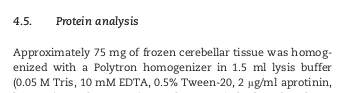
\includegraphics[scale=0.8]{fig/bad_sent_tok_1.png}
\end{center}
As one can see, the beginning of the sentence consists in an overlap of the title of the section and the paragraph following it. 

Another highly represented class of such false sentences is the result of the PDF reader reading the content of data tables in the PDFs.
Here is an example [PMID: 23022093]:
\begin{quote}
Template network Anatomical center of the difference-cluster Coordinates Volume Effect (ml) XYZNOI1 (Medial visual network) NOI2 (Lateral visual network)NOI3 (Somatosensory/auditory network)NOI4 (Sensorimotor network)NOI5 (“Default mode† network)NOI6 (executive/attention/salience network)NOI7 (Left dorsolateral visual stream/working memory)NOI8 (Right dorsolateral visual stream, working memory)Frontal pole 36 91 48 0.51 M > P Hypothalamus 45 59 30 0.49 M > P Cuneus 38 24 50 0.58 M b P Dorsocaudal anterior cingulate 45 66 60 1.32 M b P Cerebellum 55 29 24 1.31 M b P 33 33 23 1.10 M b P Amygdala 33 65 23 1.16 M b P Cuneus 44 26 52 0.85 M b P Precuneus 37 26 59 0.62 M b P Frontal pole 59 86 51 0.47 M b P Supramarginal 74 50 58 0.45 M b P Occipital pole 55 18 32 1.06 M > P Cerebellum 45 42 35 52.67 M b P White matter 53 67 45 3.26 M b P Supramarginal gyrus Right 16 43 51 2.30 M b P Left 75 42 54 0.50 M b P Insula 21 69 36 1.38 M b P Ventricle 42 47 42 0.98 M b P Premotor 38 65 68 0.97 M b P Frontal pole 59 87 48 0.60 M b P Posterior cingulate cortex 45 37 49 8.58 M b P Rostral anterior cingulate 46 90 34 8.52 M b P Frontal pole Right 29 80 59 2.79 M b P Left 58 81 58 2.49 M b P Brainstem 45 60 29 1.94 M b P Fusiform Right 36 26 30 1.58 M b P Left 53 23 28 0.84 M b P Cerebellum 66 27 14 0.97 M b P 54 42 12 0.75 M b P Lateral parietal lobule 65 28 60 0.86 M b P Retrosplenium 39 41 35 0.54 M b P Middle frontal gyrus 71 71 56 0.48 M b P Left caudate 44 63 41 1.01 M b P Dorsal anterior cingulate 45 76 46 0.70 M b P Cerebellum 57 27 17 0.46 M b P Frontal pole, right 30 90 48 0.42 M b P Insula Left 63 71 35 0.41 M b P Right 28 73 29 0.38 M b P Dorsal paracingulate 47 91 44 1.18 M > P Cerebellum 34 23 18 0.74 M > P Frontal pole Left 56 86 53 0.57 M > P Right 24 85 47 1.63 M b P Middle frontal gyrus 32 73 64 1.84 M b P Frontal gyrus Left 65 79 47 16.62 M b P Right 19 78 46 1.98 M b P Left inferior temporal gyrus 72 37 30 2.38 M b P Precuneus 45 26 60 1.46 M b P Superior parietal lobule 68 38 62 0.99 M b P Occipital fusiform 41 22 32 0.73 M b P Left hippocampus 54 55 28 0.67 M b P Retrosplenial cortex 49 42 38 0.41 M b PNOI templates are obtained from independent component analysis as described by Beckmann et al. (2005). 
\end{quote}
while in original PDF it looks like:
\begin{center}
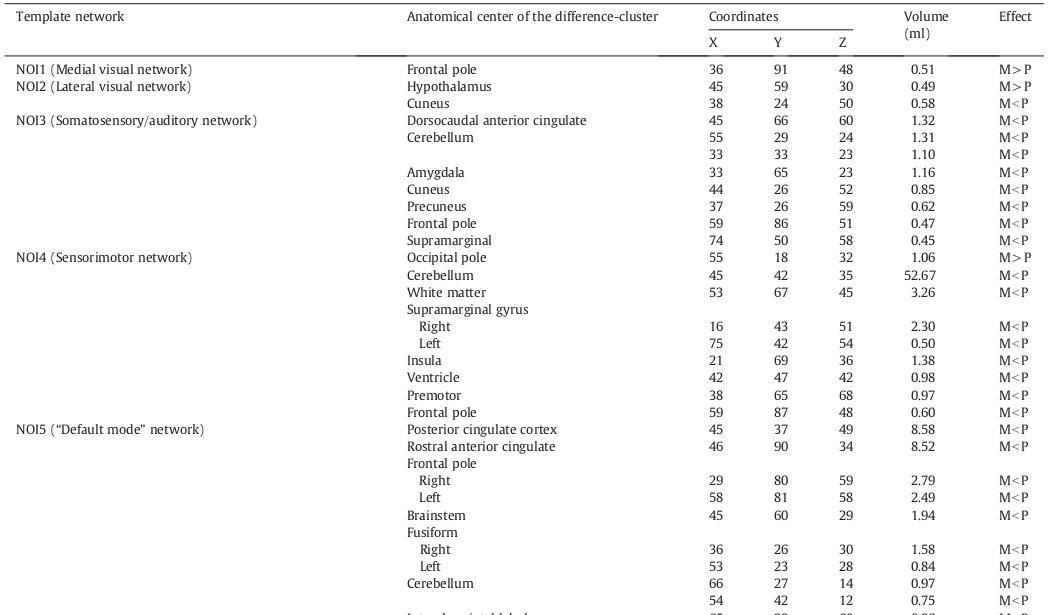
\includegraphics[width=\textwidth]{fig/bad_sent_tok_2.png}
\end{center}
Note that the above example is a good example of the hardness to treat full-text table extracted from PDF documents.
Note that these two classes of error (sentence tokenization problem and table error) are highly correlated ($r = 0.86$). It can be explained by the fact that a table error is a special instance of a sentence tokenization problem. 93\% of the cases where a sentence presents a tokenization problem, the sentence appears to be spanning a data table.
Nevertheless, a quick fix can be deduced from the fact that sentences spanning table content appear to be quite longer than normal sentence. More precisely, the indicator telling whether a
sentence has a length greater than 1000 characters has a 0.768 correlation with the one indicating that a sentence has a table form.
Note that the problems of sentence tokenization is a major problem for our 
extraction. since 71.33\% of the sentences suffers from it. That is, filtering out 
sentences whose length is greater than 1000 charcters appears to be a good 
workaround.

\subsubsection{Bad Chunking}
We talk of bad chunking when a chunk contains non related (syntactically speaking) protein and concentration.
A current pattern in the syntax of scientific literature is the use of enumeration. The co-occurrences of a protein and a concentration 
do not escape this rule. Consider the co-occurrences between biomedical entities and concentration in the following sentence [PMID: 22197517]:

\begin{quote}
Tissues were sonicated in 1\% SDS in TE (pH = 7.4) containing 1 protease inhibitor cocktail (1 mM AEBSF, 0.08 mM aprotinin, 21 mM leupeptin, 36 mM bestatin, 15 mM pepstatin A, and 14 mM E-64).
\end{quote}

Note that the number of co-occurrences grows exponentially with the length of the enumeration. Let $B$ be the set of biomedical entity appearing in the above enumeration.
That is,
$$
B = \{\text{AEBSF, aprotinin, leupeptin, bestatin, pepstatin, E-64}\}
$$
and $C$ the set of all the concentration appearing in the example. That is,
$$
C = \{\text{1 mM, 0.08 mM, 21 mM, 36 mM, 15 mM, 14 mM}\}.
$$

Then, the total number of co-occurrences in the enumeration is $|C\times B|$ when following a naive approach. To solve this misconception, one can argue that, in the model described before, the co-occurrence of a protein and a
concentration is considered as being a relation if the protein and the concentration appears in the same syntaxical chunk. However, in practice, the definition of
chunk provided by the OpenNLP chunker \cite{chunker} contains too much irregularities to assume that any enumeration would be separated on the commas. 

The problem of bad chunking seems to be present in 21\% of our results.
After excluding 
the sentences being badly tokenized from the calculations since it is hard to decide whether a piece of text is properly chunked in those since the concept of chunk only makes sense in a syntactically correct context, 
the resulting sample contains 65.1\% of cases with chunking problem. That is, we decided to add some properties to the definition of chunk, namely
\begin{itemize}
\item a item of an coma-separated enumeration is always one chunk, and
\item pattern of the form '$\langle$a protein mention$\rangle$ ($\langle$a concentration mention$\rangle$)' is always in one chunk.
\end{itemize}
Then, to avoid the combinatorial expansion of the number of co-occurrences, only the high-confidence co-occurrences are kept, namely the co-occurrences with the smallest
distance between their members. Reconsider one of the examples from section
\ref{sec:bannerM} [PMID: 15016809]:
\begin{quote}
The follicular membranes were removed by digestion in Ca2-free OR2 solution ({\color{blue}82.5 mM} NaCl, {\color{blue}2.5 mM} KCl, {\color{blue}1 mM} MgCl , {\color{blue}5 mM} HEPES, 2 pH 7.6) containing {\color{blue}2 mg/ml} {\color{red}collagenase} (Sigma). 
\end{quote}
If one consider all the 5 possibles pc-cooccurrences enclosed by the sentence, it
gets 4 false positives. However, keeping only the nearest-neighbours co-occurrence which contains ``{\color{red}collagenase}'' means keeping only the co-occurrence between it and the closer concentration in the sentence, i.e. ``{\color{blue}2 mg/ml}''. One could argue that this approach can be used among sentences and free us from using chunks. However, notice that a protein and a concentration mentions at both ends of a sentence intuitively tends to be unrelated but could be a nearest-
neighbouts co-occurrence provided no other mention of such kinds exists in the 
sentence. Therefore, we keep our approach to consider pc-cooccurrences among 
chunk, but, in the case where more than one concentration or protein occurs in a 
chunk, we use a nearest-neighbours policy.
\subsubsection{Bad Protein Mentions}
Qualitative analysis of protein estimated mentions reveals two big problems: (1)
when BannerM is run on table, it becomes unpredictable as revealed by these examples of extracted protein estimated mentions:
\begin{itemize}
    \item GR 3 19 F 5 Anisocoria  GR 4 16 M 7 GR 5 35 M 4 Anisocoria  GR 6 48 F 12 Anisocoria GR 7 28 M 3  GR
    \item C9 87 M 17 IV
    \item UI 16 2 79 F 76 3 GD
    \item LB 86 F W 16 Str 
    \item NrA Normal control C-2 80 M 12 NrA Normal control C-3 57 F 8 NrA Normal control C-4 70 M 7 NrA
    \item P Middle frontal gyrus 32 73 64 1.84 M b P Frontal gyrus Left 65 79 47 16.62 M b P Right 19 78 46 1.98 M b P
\end{itemize}
and (2) chemical elements are interpreted as protein mentions such as ``NaCL'' or ``KHPO4''.

The first problem should be overcome by filtering out the text coming from table content using the
length of sentence as explained in section \ref{sec:table_error}.
To limit the number of some obviously non-protein chemical elements BANNER considers as protein mentions, a list-based filter was built based on the more frequent of such confusions. A more long-term efficient approach would have been to use a chemical NER such as OSCAR4 \cite{oscar} to differentiate a protein mentions from chemical ones, but this would have increased the runtime too much considering the time constraint of the project.

		
		\section{Large-scale Dataset after Filtering}
		Memoization of the outputs of machine-learning-based annotators 
		using BinaryCasWriter and BinaryCasReader of the Bluima
		toolkit \cite{bluima} during the production 
		of the last large-scale dataset allows the quick production of a new dataset after inserting different filters in the 
		pipeline as described in the last chapter.
		\subsection{Filtering summary}
		To sum up what have been described above, this new large-scale run is performed with new elements in the pipeline, i.e.
		\begin{itemize}
			\item a chunk adapter as described in last section,
			\item a list-based filter to limit number of the chemical entities in
			the collected protein estimated mentions,
			\item a sentence-length filter which filters out sentences with length
			higher than 1000 characters, and
			\item a nearest neighbours co-occurrences annotator which only keeps 
			co-occurrences enclosing the closest entities --- in case of race when
			two possible co-occurrences enclose entities at the same distance of 
			each other, the first detected co-occurrence is kept.
		\end{itemize}
		
		\subsection{Reconducting the 300-records Experiment} 
		Reconducting the 300-records experiment, the experiment on error distribution conducted on the last large-scale extraction (see \ref{sec:first_300}), leads to promising result regarding
		the syntactical quality of the data. Indeed, the filtering applied during this extraction remarkably reduced the impact of the
		sentence mistokenization problem, namely only 8\% of the sentences appear to be mistokenized in this dataset and also 8\% are
		in a table form. However, chunking problems are still present in 37\% of the records but not in the form of combinatorial expansion of co-occurrences. Some
		doubts can be emitted regarding the efficacity of the chunk adapter. 
		Note that some little bugs have been diagnosed and corrected in the chunk
		adapter since; thus, the percentage of chunk error must be reconsidered.
		No new data is available at the moment. Despite the bug, qualitative analysis of the results
		seems to indicate that the quality of non-buggy chunks are better than
		in the last run. Therefore, the nearest-neighbour co-occurrences seems
		to produce good results.
		
		\paragraph{}More generally, about 60\% appears to be error-free 
		from the point of this experiment. This is a slightly good result 
		considered relatively to the first dataset which has only about 8\% of its
		results presenting none of the considered errors.
		
		
		\subsection{The apparent Lack of True Positives}
		
		\begin{table}[t]
		\begin{tabularx}{\textwidth}{|l|X|}
		    \hline
		    \textbf{Pubmed ID} & \textbf{Sentence}\\
		    \hline
		    9483526 & The rat hippocampus was homogenized (5\% w/v) in cold PBS containing 1 mg/ml of leupeptin, 
		    100 mM phenylmethylsulphonyl fluoride, and 1 unit/ml aprotinin, and centrifuged at 10,000 g for 30 min.\\
		    \hline
		    20829391 & Rat cortical neurons were serum starved for 3 d and then stimulated with 0.5 nM insulin.\\
		    \hline
		    21784010 & Hippocampus was homogenated by sonication in 250 l of lysis buffer (PBS, 1\% Nonidet 
		    P-40, 0.1\% SDS, 0.5\% sodium deoxycholate, 1 mM phenylmethylsulphonyl fluoride, 10 g/ml aprotinin, 
		    1 g/ml leupeptin, 2 g/ml sodium orthovanadate) and centrifuged at 13,000 rpm for 15 min 4 $^\circ$C.\\
		    \hline
		    15896913 & Dissected hippocampus was homogenized in lysis buffer (18 l/mg tissue) containing 137 mM 
		    NaCl, 20 mM Tris?HCl (pH 8.0), 1\% NP40, 10\% glycerol, 1 mM PMSF, leupeptin (1 g/ml), sodium vanadate 
		    (0.5 mM), AEBSF (100 mg/ml).\\
		    \hline
		\end{tabularx}
		\caption{Some example of the ``methodological pollution''}
		\label{table:extrSent}
		\end{table}
		In addition to make the data cleaner, one of the aim of this second 
		large-scale data collection was to diminish the persistent hardness to
		find instances of the targeted relations\footnote{Reminder: the relation 
		describing how a given protein is concentrated in a given location (all 
		scale included: cellular, subcellular, regional). See section \ref{sec:project_desc} for more details.} among results. 
		
		The apparent majority of the results, in spite of their clearly better 
		quality than in the first large-scale run, comes from the 
		\textit{Materials and methods} section or are, at least, methodological 
		data which is not the main concern of BBP researchers. That is, they 
		describe experimental process which is not the most wanted kind of 	
		relations in the perspective of this project. Table \ref{table:extrSent} shows some examples of  such 
		sentences. The rarity of true positives could also indicate that our 
		focus on brain region as the third entity of our co-occurrences is wrong 
		regarding to the desired information. That is, some focus on the cell 
		types and subcells data is important at this stage. However, a 
		qualitative inspection of the records for the cellular scale reveals that the ``methodological polution'' of our data is still there. For instance,
                this extraction counting 286100 records, filtering out the sentences containing lemmas that are typically methodological, 
                namely ``incubat'', ``wash'', ``culture'' or ``buffer'', results in a set of 181122 records. That is, 104978 have been filtered out
                by such an approach. Note that this kind of filter can be damageable without a corpus to evaluate them. Therefore, we tried
                to apply a more conservative approach. First, the section title are annotated using a regexp approach. Then, a confidence flag is added to each record
                having a higher value if it corresponds
                to a sentence in a section like \textit{Results} or \textit{Conclusions} and a lower one if it corresponds to a sentence in the 
                methodological section(s). If it is not possible to determine the section enclosing a sentence, then a neutral confidence flag is set.
                The first qualitative look at the resulting materials (after section-confidence annotation)
                seems to show that
                \begin{itemize}
					\item indeed, the resulting data is more result-oriented and, that is, more useful to researchers,
					\item it seems that a considerable number of methodological mentions still appears in the sections presenting results in the papers 
                and, therefore, does not solve the problem, and
					\item the targeted relation still appears to be hidden.
                \end{itemize}
                
                
		
		
		\section{Results overview}
		
			The summary of our final results are shown in table \ref{table:result_summary}. It intends to give
			an overview of the results obtained for the three considered scales (brain region, cell and subcell). The 
			first row shows the number of records extracted for each scale. The next rows display the size of some 
			interesting subsets of our final dataset. 
			Finally, the two last rows respectively shows the percentage of the data 
			extracted from a section presenting results (\textit{Results}, \textit{Discussions}, \textit{Conclusions}) and from the 
			\textit{Materials and Methods} section. Note that the fact this two rows do not sum up to 100\% is due
			to the cases where it is not possible to establish the section from which they were extracted.
			
			\paragraph{}As a conclusion for this chapter, it is interesting to see that, even if the methodological pollution
			is effective in our data qualitatively speaking, our extractions comes more from the section about results
			than from the methodological sections in general. This seems to confirm the qualitative conclusion of last
			section concerning the presence of methodological content in the sections about results and, therefore,
			challenges the chosen approach to classify sentences as being methodological or not. Finally, a web application
			has been developed to make the result avaible and is described in next section.
			
\begin{table}[h]
\begin{tabular}{|l|l|l|l|}
\hline
\textbf{Scale}	&\textbf{Brain region}	&\textbf{Cell}    &\textbf{Subcell}\\
\hline
\textbf{\# records}	&41'938	&286'100	&2'255\\
\textbf{\# distinct triplets}	&37'212	&166'371	&1'844\\
\textbf{\# distinct proteins}	&18'431	&75'101	&1'295\\
\textbf{\# distinct regions/cells/subcells}	&7'808	&488	&57\\
\hline
\textbf{\% from RESULTS}	&48.60\%	&48.50\%	&57.80\%\\
\textbf{\% from MM}	&28.50\%	&32.40\%	&17.90\%\\


\hline
\end{tabular}
\caption{Final result summary}
\label{table:result_summary}
\end{table}
			 
		\chapter{Visualizing the results}
		
			This chapter summarizes the visualization tool developed to present the results
			of this work to BBP researchers. A server which makes the collected data
			avaible in JSON form was developed in Python using the Tornado 
			framework\footnote{See \url{http://www.tornadoweb.org/en/stable/}.} and follows a REST-full philosophy.
			In addition, three views were developed in HTML/CSS/JavaScript using Bootstrap framework\footnote{See \url{http://getbootstrap.com/}.} to visualize
			the collected data. The next sections intend to give an overview of each of those.
			
			\section{The Top Table View}
			
			The Top Table View displayed in figure \ref{fig:tt_view} 
			intends to allow the researchers to quickly access the
			details concerning the most frequent triplets through a color-coded 
			table. It confronts the most frequent proteins and the most frequent
			brain regions (it can easily be adapted for cells or subcells too) in
			a table and displays in the cells how many relations exists between them according
			to our dataset. The cells are color-coded following the principles: 
			the darker, the more. Once set up on a Tornado server, the Table
			View is accessible by GETting /static/table.html.
			\begin{figure}[h]
				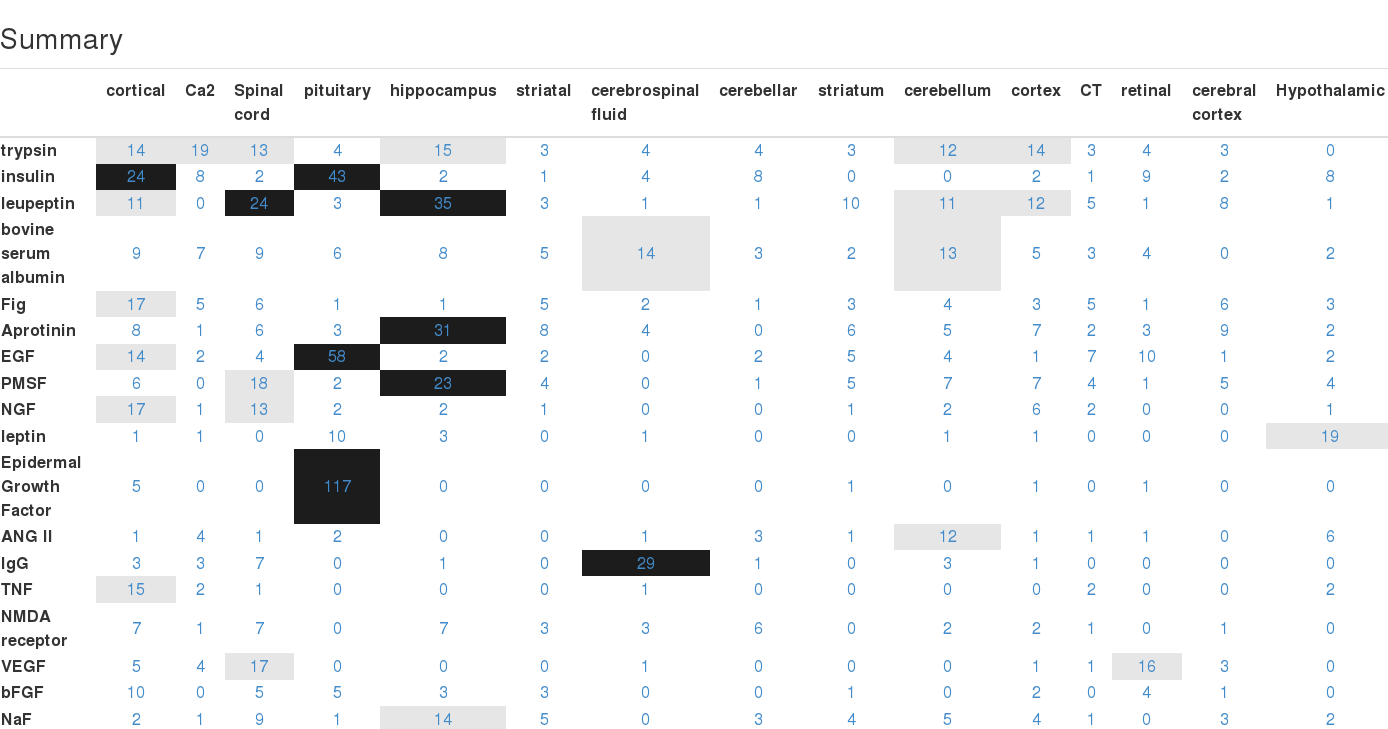
\includegraphics[width=\textwidth]{fig/top_table_view_screenshot.png}
				\caption{A screen shot of the Top Table View}
				\label{fig:tt_view}
			\end{figure}	
			
			\section{The Search View}
			
			As one can see on figure \ref{fig:search_view}, the Search View intends to allows
			a more specialized access to the data by letting the user enters keywords for the protein
			or brain region (exact match or SQL regexp) according to its interest. The search results 
			are then displayed in a list mode and are sorted according to the amount of data avaible
			for each of them. To illustrate the different keyword matching: 
			searching for protein ``insulin'' in exact match will returns
			only relations involving insulin while searching for ``\%insulin''
			in SQL regexp (LIKE syntax\footnote{See \url{http://dev.mysql.com/doc/refman/5.0/en/pattern-matching.html} for references.}) returns relations involving ``insulin'',
			``bovine insulin'' and ``plasma insulin''. The Search View is
			accessible by GETting /static/search.html.
			
			\begin{figure}[h]
				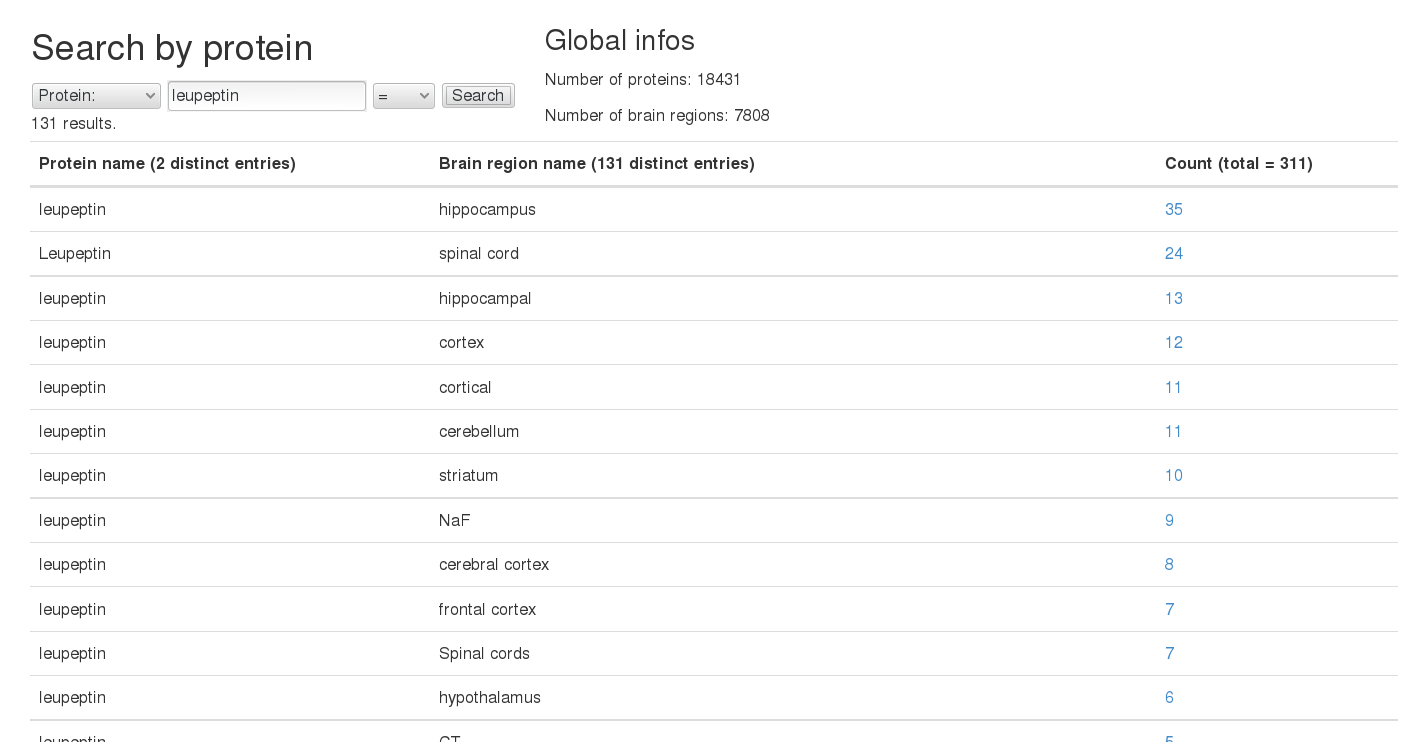
\includegraphics[width=\textwidth]{fig/search_view_screenshot.png}
				\caption{A screen shot of the Search View}
				\label{fig:search_view}
			\end{figure}
			
			\section{The Detailed View}
			
			The detailed view can be accessed either from the Top Table View or the Search View. It displays
			the collected data in plots for normalized concentrations and in tables for unnormalized information as displayed on figure \ref{fig:detailed_view}.
			It also provides a quick way to access the original document by providing a link to its PubMed citation
			after the user has clicked on a data point as shown in figure \label{fig:detailed_view_2}. The plots
			are drawn using the AmCharts JavaScript library\footnote{See \url{http://www.amcharts.com/}.} and displays, for a given concentration on the
			$x$ axis, the number of such concentration for the relation in 
			question on the $y$ axis. For instance, the Detailed View for the 
			leupeptin protein and hippocampus brain region displays the data 
			point $(1,3)$ in the plot for kg/m$^3$-normalized units meaning that
			our databases contains three relations linking 1 kg/m$^3$ of leupeptin 
			and hippocampus.  
			\begin{figure}[t]
				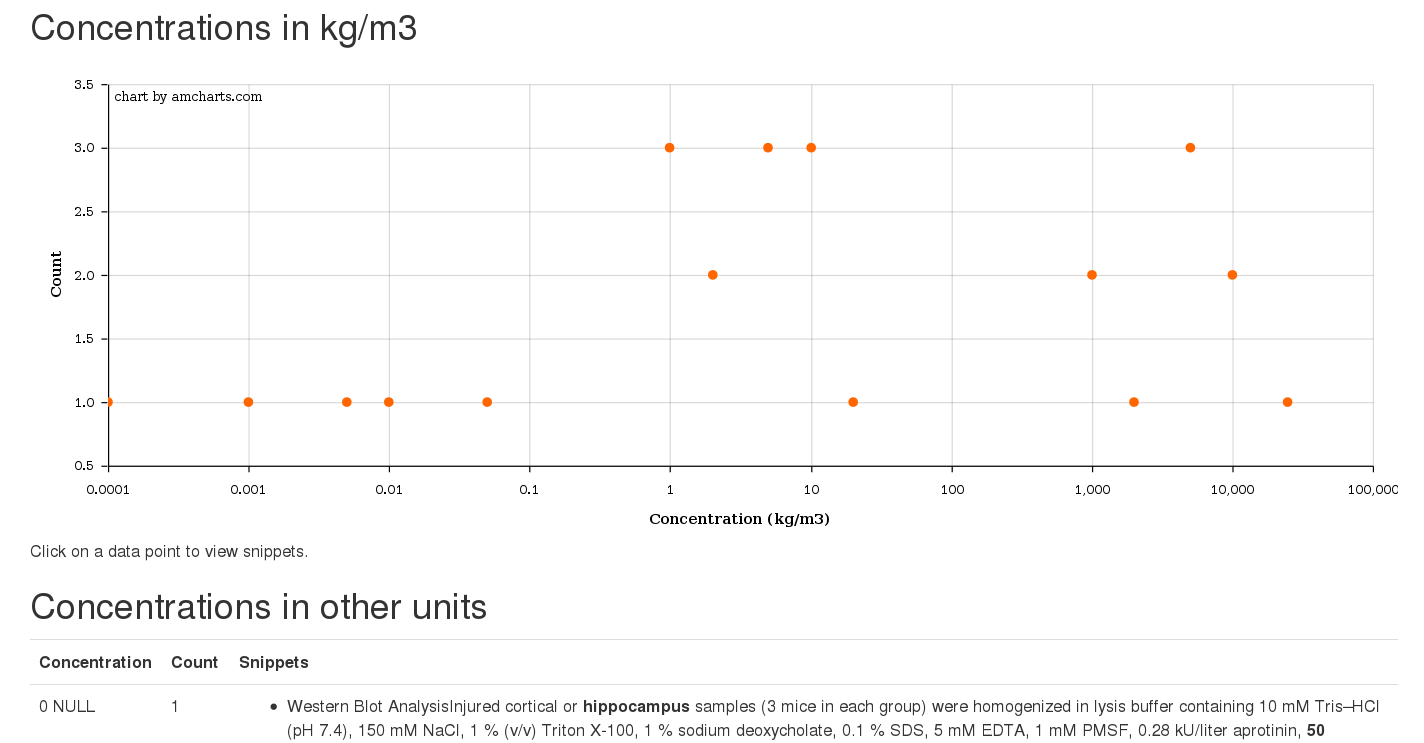
\includegraphics[width=\textwidth]{fig/detailed_view_screenshot.png}
				\caption{A screen shot of the Detailed View}
				\label{fig:detailed_view}
			\end{figure}
			\begin{figure}[b]
				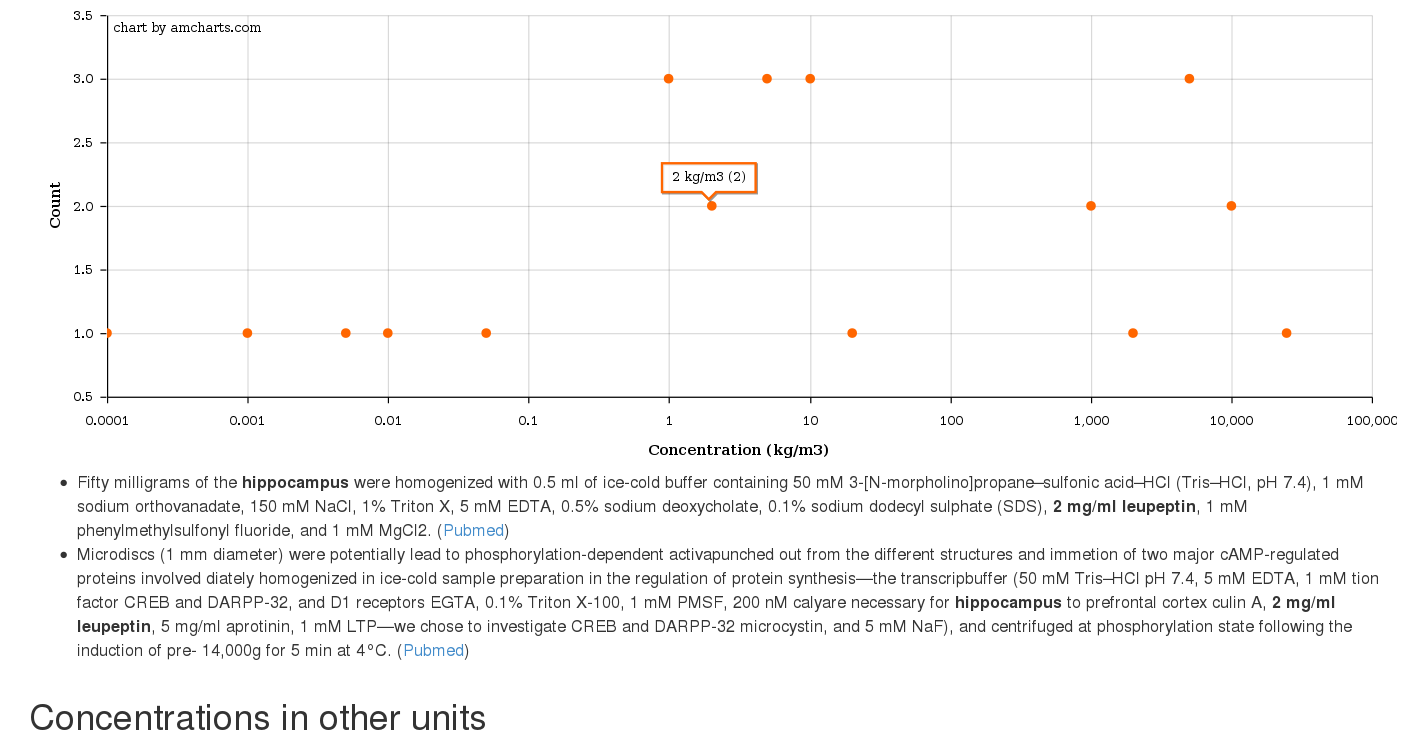
\includegraphics[width=\textwidth]{fig/detailed_view_screenshot_2.png}
				\caption{A screen shot of the Detailed View once clicking on a data point.}
				\label{fig:detailed_view_2}
			\end{figure}
			
			
			\addtocontents{toc}{\protect\enlargethispage{\baselineskip}}
                \chapter{Conclusion}
                \label{chap:conclusion}
				%OUTLINES:
				%- RELATIVE SUCCESS
				During this work, we have seen that
				\begin{itemize}
					\item 	the extraction of relations linking a protein, its concentration and a brain location
							can be performed using simple heuristics associated with powerful existing NERs despite the very
							specific nature of this material
					\item	but attempting to select the targeted relation
					kind (how concentrated is a given protein in a given
					location) among the results seems to remain hard. 
				\end{itemize}
				
				The heuristics used in this project seems not to be enough
				efficient to overcome the lack of reference annotated 
				corpus. But only future researchers' feedback will be able to 
				establish the usability of the current dataset.
				To overcome the difficulty to classify the strength of the collected relations, this project 
				could constitute a basis to construct a reference annotated
				corpus through, for instance, an active learning tool for making
				the classification of the relations more precise. In this 
				perspective, a visualization displaying the results has been 
				developed and will be made available to researchers
				for feed-back and, then, for evaluation. 



				
				%- WHERE IS THE VERY DATA HIDDEN
				\paragraph{}The question of where the targeted relations are is still open at this stage.
				The rarity in the results of our extractions of the very specific relations characterizing the concentration of a protein in a location of the brain 
				(all scale included: regional, cellular, subcellular, ...) challenges an assumption implicitly supported
				along this project that such relations can be extracted from, or even found in the body of scientific publications. This guess
				has been made not merely because of the absence of corpus to evaluate such assumption but because of the lack of
				tools to properly treat other form of data presentations in paper in PDF format including charts and 
				tables\footnote{the example given in section \ref{sec:table_error} bears witness of the hardness to use full-text
				table using the current version of the tools}, development of whose
				was outside the scope of this project. Therefore, future work attempting to extract highly specialized data 
				could focus on the treatment of such data formats. One could also ask, more generally, if the very targeted relations really exists in scientific literature. Another future work could be to use the pseudo corpus we produce (by annotating sentence as belonging to the methodological section or to the section presenting results) to bootstrap a reference corpus regarding the classification of sentence as being semantically methodological or not. 					
				%- BLUIMA IMPROVEMENT
				\paragraph{}Finally, one of the successfully reached goal of this project is its contribution to the improvement of the Bluima toolkit  \cite{bluima}
				especially regarding the addition of tools dedicated to relation extraction (in particular improved co-occurrence extractors),
				some of which are currently already in use in other project(s) supported by the BBP.	
				
			\section*{Acknowledgment}
			
			This project was realized in the context of the Blue Brain Project.
			
			\paragraph{}
			I would like to express the deepest appreciation for my supervisors: Jean-C\'edric Chappelier for sharing 
			its scientific rigour, its experienced advices and support as well as its availability for constant follow-up, 
			and Renaud Richardet for its advices, its impressive availability, its participation to all the steps of this 
			project and its technical support.
			\paragraph{}
			I also place on record my sincere gratitude to Martin Telefont and Daniel Keller for their participation
			and feedback.

		\bibliographystyle{plain}	
		\bibliography{refs}
\end{document}	
